\documentclass[11pt, twoside, reqno]{book}
\usepackage{amssymb, amsthm, amsmath, amsfonts}
\usepackage{graphicx}
\usepackage{color}
\usepackage{url}
\usepackage{hyperref}
\usepackage{verbatim}
\usepackage{ wasysym }
\usepackage[toc,page]{appendix}
\appendixpageoff
\usepackage[leftmargin = 1in, rightmargin = 0in, vskip = 0in]{quoting}
\usepackage{microtype}
\usepackage{bardtex}
\styleoption{seniorproject}
\usepackage{listings}
\definecolor{codegreen}{rgb}{0,0.6,0}
\definecolor{codegray}{rgb}{0.5,0.5,0.5}
\definecolor{codepurple}{rgb}{0.58,0,0.82}
\definecolor{backcolour}{rgb}{0.95,0.95,0.98}
\lstdefinestyle{mystyle}{
    commentstyle=\color{codegreen},
    keywordstyle=\color{magenta},
    stringstyle=\color{codepurple},
    basicstyle=\ttfamily,
    backgroundcolor=\color{backcolour},
    frame=lrbt,
    breakatwhitespace=false,      
    framexleftmargin=8pt, 
    framexrightmargin=8pt,   
    framextopmargin=6pt,
    framexbottommargin=6pt,
    breaklines=true,                 
    keepspaces=false,                 
    numbersep=0pt,                  
    showspaces=false,                
    showstringspaces=false,
    showtabs=false,                  
    tabsize=1
}
\lstset{style=mystyle}
\newcommand{\blockquotespacing}{\blockspaced}
\newcommand{\prose}{.25in}
\newcommand{\poetry}{0in}
\newcommand{\singlespaced}{\setstretch{1}\vspace{\baselineskip}}
\newcommand{\blockspaced}{\setstretch{1.3}\vspace{\baselineskip}}
\newcommand{\doublespaced}{}
\newenvironment{blockquote}[1][\prose]{\setlength{\parindent}{#1}\begin{quoting}\blockquotespacing}{\end{quoting}}
\begin{document}

\titlepg{Shifting Tone of a Body of Text}{Cole Hollant}
    {May}{2020}

\abstr
We will be looking into altering the tone of a body of text based off of Robert Plutchik's basic emotions while preserving the original meaning. This project encompasses building probabilistic models in the realm of natural language processing (nlp), full-stack web development, dataset creation and application, along with proofs of algorithmic runtimes. We will build our models off of latent Dirichlet allocation—a grouping model common in nlp—and may explore neural networks as a means of emotion recognition. This will also involve user testing as a means of measuring the effectiveness of our models as well as guiding the development cycles.

\tableofcontents

% \dedic

% Text of dedication.

% \acknowl

% Text of acknowledgments.

\startmain

% \intro

% Text of Introductory Chapter.

\chapter{Thesaurus Write Up}
% <!--
% Summary of this file:
% - I need a thesaurus because we are going to be swapping words for ones with similar meaning
% - I want to have my own because of manipulating data, cost, and the learning experience
% - We web scraped it!
% - Picked words.bighugelabs.com because it was cool with being scraped and it had what we needed!
% - Practically anything can be used for webscraping so long as you have requests and string manipulation
% - We used bs4 and requests, and we wrote by first letter
% -->


\section{Why do I need a thesaurus?}

A moldable thesaurus is seemingly very important for my project. I'm looking at building a model to shift the tone of a body of text while attempting to preserve semantics. Simply going off of intuition, we can figure that swapping a word for a synonym of that word may alter the tone of its enclosing sentence. Consequently, we would like to aggregate some relative relationship between some set of tones and groups of synonymous words. Upon creating such a dataset, we may interchange a word with a synonym according to a difference in tone.

\section{Why not use an existing API?}

There are a few reasons to construct or reconstruct our own thesaurus. First and foremost, we are interested in keeping additional data regarding tone that is not present within existing thesaurus APIs. It is far easier to manipulate data if it is all on hand, and it should save some server-side complexity in dealing with the decoupling of the thesaurus and the word-tone relationships. There is an issue with cost as well: APIs are rarely free past some established number of calls in a given time interval, and I would like for this software to function with minimal cost--ideally the only cost is in hosting. Finally, this is a project in the realm of software engineering. While it is often better to rely on existing services--standing on the shoulders of those who came before you--it is also important to know how to create your own services.

\section{How did we do it?}

We created the thesaurus by web scraping, which is a large aspect of data-collection and thus is often a necessity in the sphere of machine learning. Of course, it is possible to compile a thesaurus using other means--surely one could buy a physical thesaurus and type up all the entries or even automate such menial tasks with computer vision--but we are interested in constructing a thesaurus as painlessly as possible. It is only one aspect of our project after all.

\subsection{Choosing a site}

Web scraping often comes with a give and take. There are several existing online thesaurus services, so we did looked into a few of them and landed on \href{https://words.bighugelabs.com}{John Watson's Big Huge Thesaurus}. We began with trying \href{https://www.thesaurus.com}{thesaurus.com}, but they have protections against traditional scraping. There are many of such protections including lazy-loading content, providing fake data, services like Captcha, even automatically altering the page's HTML. It seemed as if \href{https://www.thesaurus.com}{thesaurus.com} had been randomizing their CSS classes and either lazy-loading content or providing fake data. While we could likely get around this with an automated browser like \href{https://www.seleniumhq.org/}{Selenium}, as the CSS classes are only a deterrent if scraping over a large time interval and the content would almost certainly exist within an automated browser session, we should respect that this site has practices in place to prevent scraping.

There may be protections against web scraping in place that we ought to honor, or there are often poorly laid out websites that would be a pain to use despite being open source, or the site may simply not provide all the information we would like. The latter is best exemplified by \href{http://moby-thesaurus.org}{moby} which we may come back to if we decide that we care not about parts of speech. \href{https://words.bighugelabs.com}{John Watson's Big Huge Thesaurus}, on the other hand, seems to have all that we want: synonyms by part of speech, a clean interface, and permission for use given credit is provided.

\textit{Protections against web scraping from \href{https://github.com/JonasCz/How-To-Prevent-Scraping/blob/master/README.md}{JonasCz}}

\subsection{Scraping the site}

Web scraping for purposes such as gathering content from a page is a basic process: get the raw HTML of the page and retrieve what you want. Due to the ubiquity of HTTP requests and string processing, we can use just about anything we want for building our scraper. We will be using Python for its simplicity in our project, although we will create something similar in a bash script as a proof of concept for demonstration (see \texttt{thesaurus/webscrape/scrape.sh}).
% <!-- Note: I dont like how this reads, but I do like having the bash script to drive the point home -->


We are using the \texttt{requests} module to get the HTML for each page and \texttt{bs4} for our HTML parsing. I am running Ubuntu on my computer, and thus have access to the \texttt{words} file present across Unix operating systems: this is a raw text file with a collection of words separated by line. This will be the basis of our thesaurus. We will first reduce this file by removing all entries with apostrophes with \texttt{thesaurus/webscrape/fixWords.py} whose essence is:
\begin{lstlisting}[language=Python]
if word.find("'") == -1:
    outfile.write(word)
\end{lstlisting}

We do this as to eliminate repetition in our database to expedite searching as all nouns present in \texttt{words} have a possessive form; note that this does come with the loss of conjuntions. Now that we have the words we will use to construct our thesaurus, we may do exactly that. Each page takes the form of the same base url followed by the word: this makes for easy access. We go through word-by-word in our reduced file, make a GET request for that word, and then aggregate all the word's synonyms and antonyms by part of speech. There's just one little trick to this process: the antonyms are not in a concrete section, but rather one of several possible subsections under each part of speech. To circumvent this issue, we just have to do some checks to make sure that any present antonym section belongs to the part of speech we are considering and not a later-occuring part of speech. We allow the addition of antonyms to the synonym list and remove them prior to returning; this allows for us to have less rigorous checks in adding synonyms.

There was an earlier version of this scraper that did not deal with antonyms. This catch is attributed to Ariadne, who—when I showed her my progress—brought up the word ``beautiful'' which had ``ugly'' as the first entry under the synonym section. This prompted quite a refactoring, and we should now be free of these bugs. The basis of this refactoring was largely tested against ``beautiful'' and ``well'' which both have antonyms in the thesaurus, and ``well'' had all the parts of speech.

Upon tweaking our scraper to suit our needs, we must output our results. As I only have so much RAM, and Python can be rather resource hungry, we segment our data by first letter. We will restructure our data into one object, but we will do this after collecting all of our data. We may naively write each dictionary to its corresponding JSON file and correct the result. This allows us to keep less in memory, which may otherwise present itself as a problem. This also allows us to segment our program as a failsafe; if we are to lose connection, crash, hit a request limit, or otherwise fail to run the script to completion, we may easily start again from where we have left off rather than the very beginning.

Then, upon building our thesaurus, we may move to the next part of our project. We would like to store this thesaurus in a database and create an API to interface with it.

\chapter{Server Writeup}

\section{What's all this then}
% <!-- revisit this garbage -->


I'd like to keep all the thesaurus entries in a database, and be able to interface with that via some API. While we could do everything locally and save some of the configuration headache, we also would hardly be able to use it. So, in the pursuit of functionality, we'll need a server to put this on.

\section{IaaS vs PaaS vs SaaS}

We had some options for this project in terms of hosting, as we have decided that we aren't in the business of including \texttt{Make} in our distribution strategy. These options come as a slew of acronyms: IaaS, PaaS, and I suppose some bare metal solution from my pockets. The last option would consist of some computer sitting in my dorm room, running 24/7, along with some router configurations that might have BardIT coming after me; the other's are the real contenders. There's a certain balance between PaaS (Platform as a Service) and IaaS (Infrastructure as a Service), each with some pros and some cons. IaaS is a rather simple option: it is as close to the bare-metal (often called ``on-premises'') solution as possible, where we would pay for some virtual machine (VM) and networking. With IaaS we are leveraging server farms, and are more-or-less renting a server. PaaS is more nuanced, as it plays a role between IaaS and SaaS (Software as a Service, like Google Apps, Dropbox, etc.), and tends to abstract desirable aspects of IaaS such as security, metrics, DNS, and so on.

We ultimately went with IaaS—for a few reasons—via \href{https://www.digitalocean.com}{DigitalOcean}, a popular cloud services platform among other names like AWS and Azure. This gives us the advantage of having all our services in the same place as opposed to the spread out nature of PaaS. There are exceptions to this heuristic, such as Openshift and other CaaS (Containers as a Service) platforms, that would allow us to keep centralized services, but pricing is one of the biggest sellers for our use of IaaS. We lose some of the ease of scalability, but that is not an aspect that we are terribly concerned with while developing the core of the project. As cash is king, we will get our hands dirty with SSL, proxies, and other niceties that PaaS would shield us from.

\section{Don't be root!}

It should go without saying that it's wise to stray from doing all things as \texttt{root}. As default, we can only \texttt{ssh} into \texttt{root}, so we must add a user! We'll still need root access, so we'll be sure to add our new user to the \texttt{sudo} group. Then to finish this setup, we must patch up our \texttt{ssh} configuration: we want to \texttt{ssh} into the new user and disable \texttt{ssh} into \texttt{root}.
% <!-- maybe remove this snippet... -->

\begin{lstlisting}[language=sh]
ssh root@<IP_ADDRESS>
adduser <USERNAME>
usermod -aG sudo <USERNAME> 
rsync --archive --chown=<USERNAME>:<USERNAME> ~/.ssh /home/<USERNAME> 
vim /etc/ssh/sshd_config    (set "PermitRootLogin" to "no")
\end{lstlisting}

Of course, we'll make a nice \texttt{ssh} config on our personal machine for our convenience. We'd like to save the hassle of keeping track of IP addresses and users and keys, so we'll make another entry to be able to simply run \texttt{ssh sproj}.

\section{The big whale upstairs}

There is certainly a warranted section on Docker. Docker is the Kleenex of containers: it's a wildly popular open source project creating, distributing, and running containers. Cointainers are an industry-molding alternative to virtual machines for running system-agnostic programs. If you've written software in the past few years, you've almost certainly seen some sort of depiction of the difference between virtualization and containerization, but in case you haven't, we can go into it. First off, the picture as promised:

\begin{center}
  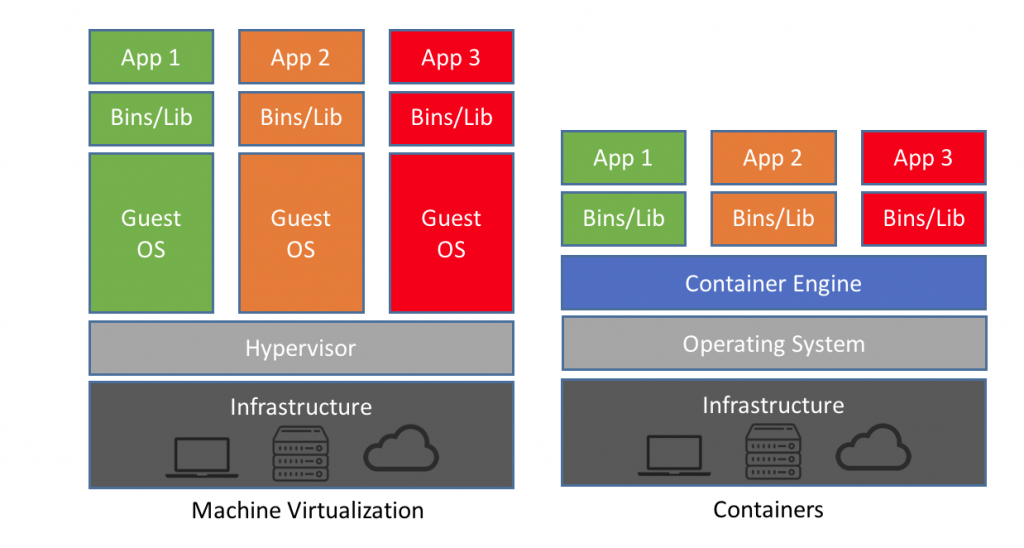
\includegraphics[width=125mm,scale=0.5]{dockerImage.png}

  {\small \href{https://blog.netapp.com/wp-content/uploads/2016/03/Screen-Shot-2018-03-20-at-9.24.09-AM-1024x548.png}{\textit{Dockerization vs Containerization}}}
\end{center}

While a picture is worth a thousand words, a picture with words may warrant a few extra. On each side we have a layer of apps on top of their dependencies that is running on top of some infrastructure. The apps and bins/libs are our binaries/executables/processes along with their source-code/libraries/etc that we are used to writing and running in our day-to-day as programmers. The infrastructure is just that: the silicon and bare metal that we are running on top of. That surmises the local development experience, and I'll trust you are familiar with the woes of your program working like a charm on your personal machine, but playing anything but nicely when you have to run it on another computer.

The ``it worked on \textit{my} computer'' dilemma is what virtualization and containerization are here to address. If we can encapsulate these processes and dependencies and abstract them from the contents of the machine they reside in, we should have platform-independent programs. Virtual machines tackle this by building entire guest operating systems on top of a hypervisor (also known as a virtual machine monitor), which serves to channel access to hardware and thus allow for multiple operating systems to run on one host operating system.

However, operating systems are quite large, and there is a lot of waste with virtualization. With the industry going towards cloud computing, we needed smaller, faster solutions. Containerization seeks to leverage the host operating system, and rather than keep several guest-os instances, we have a single container runtime environment.
% <!-- This has to go... -->


It's a similar solution to that which the JVM provided in the 1990's. And, since I couldn't help but mention the JVM, I can't stop myself from mentioning that there's great interest in scrapping it in the context of containerization: if we are running in containers, do we need to keep the JVM around? JetBrains is producing Quarkus for doing ahead-of-time compiling for making Java more container-friendly. More container-friendly is--of course--a euphimism for ``Java containers are gigantic and slow'': while even an amateur can get containers down to a handful of megabytes (the beginnings of my frontend, proxy, and api are all just about 20MB), it's quite rare to see a Java image less than around 80MB.

This may not seem like a big deal, we are only talking on the order of megabytes. But in the days where serverless architecture/microservices are growing in popularity, there is an ever-increasing need for quick cold-start times (starting an idle container, should none be active and available). Serverless computing being a platform in which cloud providers provision your resources, and the customer is charged for active time rather than paying for a more traditional flat-rate server. This is attractive as it isn't wasteful, but if a request is made, there's always a chance that your containers are down, and they must be reinitialized to fullfill the request. If we can optimize our containers, we'll save time, money, and our user-experience!

This tangent on a direction the software engineering industry is headed ought to demonstrate the appeal of containers: serverless wouldn't even be a fever dream if we only had VMs.

\subsection{Building My Containers (Thesaurus)}

With containerization, the name of the game is modularity. So, we generally aspire to have per-process containers. Thus my one web app comprised of a frontend, a database, a CRUD-wrapping API, a model API, and a server/reverse-proxy has five containers: one for each aspect. And with inter-container dependecies, one would think that things would get confusing. This is where docker-compose comes in. This is a tool that allows for the definitions/instructions for multiple containers. This is a dev-ops dream, where I can deploy my application with a single command (and preserve my volumes!). It's configured in a \texttt{yaml} file and maps nicely to standard docker cli arguments: we specify things like \texttt{Dockerfile} location, port forwarding, networds, container dependencies, volumes, environment variables and more!

I'll touch a bit on how I made my various containers, and then configuring my compose file. It's far simpler than it sounds.

\label{Go CRUD Backend Dockerfile}

Golang compiles to binaries per OS, which is excellent news for us! If we can compile to binaries, we don't need to keep all the installation business around, so we simply copy over the source code, install the packages, and compile as a build stage. Then, we can copy over the executable to a smaller base image, expose our port, and run! It's a process similar to a writing standard shell script, and we are generally concerned with the resulting size. This was an example of a multistage Dockerfile, where we separate the compilation stage from the runner stage; this is quite common as a measure of reducing image size.

\label{Python Model Backend Dockerfile}

The Python dockerfile is rather plug and play as we aren't doing anything too fancy like using Cython; we are just using plain old 3.7 Python. We extend the Python 3.7 Alpine image (Alpine being a remarkably small linux distribution), make our working directories and copy over our files as usual. Then it's just a matter of installing everything in our \texttt{requirements.txt}, exposing a port, and running in module mode, as we might expect. There are other strategies for reducing Python containers, like \texttt{pip install}-ing your code base as outlined \href{https://pythonspeed.com/articles/multi-stage-docker-python/}{here}, but the Python container is already small enough for our satisfaction where the simpler single-stage option is just fine. If we were to move toward the world of lambdas, we may reconsider, but we will settle for now.

\label{Vue Frontend Dockerfile}

The dockerfile for the frontend is similarly simple. We copy over the source code, install all the dependencies, and build our app. Then we follow our Golang footsteps and run from a smaller nginx image. This is a good point to mention the repetition within many Dockerfiles; you may note that we are separating installing the Vue CLI tools from installing all the node dependencies. This is because docker gives intermediate image tags per layer (each line in the Dockerfile), which we may run from.

\label{Mongo and Nginx}

The MongoDB and Nginx containers are as easy as can be. We simply change nothing from the base images! This is part of the beauty of being a part of a vibrant open source community.

\label{The Composition}

Within our docker-compose file, we naturally define a service for each previously mentioned aspect. The common bits are that each service is given the location of the Dockerfile or image, all are set to restart unless-stopped (as I will just be deploying a single instance of this), each is given a pseudo tty in case anything goes a-muck, everything is given some sort of port mapping, and everything is added to a network. Outside of this, we link the backend to the database, and we are good to go! From here we can build our little cluster and tear it down at will.

Since this deployment is in essence a personal project (I hardly expect more than a handful of people to check it out in these stages), I'm not concerned with auto-scaling and load-balancing. Should the need arise, everything is fully containerized, and it is just a matter of migrating to a container orchistration platform like Kubernetes.

\chapter{Lexicons}
% <!--
% Questions:
% - what exatly is word-sense? is it [this](https://en.wikipedia.org/wiki/Word-sense_disambiguation)
% - Answer: from wikipedia "Words are in two sets: a large set with multiple meanings (word senses) and a small set with only one meaning (word sense)"
% -->


\section{National Research Council Canada (NRC) Emotion Lexicon}

\subsection{IMPORTANT NOTE: remember to cite as per Terms of Use in their readme}

This is the lexicon that we are most interested in as it is most directly related to our project. There are two forms of this lexicon: the ``word-sense'' lexicon is the original annotated at the word-sense level and the ``word'' lexicon is a baked version which condenses all word-senses for a word.

We've made some mistakes in the past, so we want to check our restructured data; if we know that the ``word-level'' form was created by taking the union of the affect associations of the ``sense-level'' form, we can create our own version of the ``word-level'' and compare the two versions. As there's little sense in keeping our own version around, we may check it algorithmically.

\subsection{Methodology}

Saif M. Mohommad and Peter D. Tourney compiled this lexicon with crowdsourcing through Amazon's Mechanical Turk (an online crowdsourcing platform); they chose crowdsourcing as it is quick and inexpensive (costing them \$2100 for the Turkers). As a deterrent of bad responses, they included a filtering question in each survey that asked for the best synonym for the given word, allowing them to identify either lack of word knowledge or probabilitically filtering random responders. They selected joy, sadness, anger, fear, trust, disgust, surprise, and anticipation as per Robert Plutchik's wheel of basic emotions, as well as drawing from the present emotion lexicons WordNet Affect Lexicon, General Inquirer, and Affective Norms for English Words and both the Maquarie Thesaurus and Google's N-Gram corpus. They generated questions with the Macquarie Thesaurus with the aforementioned filtering-question followed by questions asking for alignment with the various emotions. They also included polarity (positive vs negative valence) in the lexicon, giving us 10 categories to work with.
% <!-- Maybe delve into Plutchik? -->

\section{Our Representation}

We wanted to preserve their data, but bring it into our database (MongoDB). This transfer was relatively painless, as their lexicon was in consistent TSV. We borrowed a decent amount of JSON utilities and structure from our thesaurus-scraper, writing to files by first letter as we go; all that changes is the shift from making http requests and parsing HTML to loading a local file and parsing TSV. We did this for both the ``word-level'' and the ``sense-level'' forms resulting in the following schema:

\subsection{Word Level}
\begin{lstlisting}[language=Python]
{
  "<word>": {
    "associations": [
      "<list",
      "<of>",
      "<associations>",
    ],
    "word": "<word>"
  },
  ...
}
\end{lstlisting}

\subsection{Sense Level}
\begin{lstlisting}[language=Python]
{
  "<word>": [
    {
      "sense": [
        "<list",
        "<of>",
        "<synonyms>",
      ],
      "associations": [
        "<list",
        "<of>",
        "<associations>",
      ],
      "word": "<word>"
    },
    ...
  ],
  ...
}
\end{lstlisting}

\subsection{Word-Sense Level}

Note that the sense-level scheme consists of arrays whose entries resemble the word-level scheme along with a field representing the word-sense; this is because the word-level representation of a word is created from the union of the sense-level entries for that word.

\begin{quote}
The original lexicon has annotations at word-sense level. Each word-sense pair was annotated by at least three annotators (most are annotated by at least five).
\end{quote}

\begin{quote}
The word-level lexicon was created by taking the union of emotions associated with all the senses of a word.
\end{quote}

\begin{quote}
— Saif M. Mohammad and Peter D. Turney (from NRC-Emotion-Lexicon-v0.92/readme.txt)
\end{quote}

Each entry from these forms can then be easily POST-ed to our API and can be accessible!

\subsection{Other lexicons}

The other lexicons that we are using are the National Research Council Canada (NRC) Colour Lexicon, Affect-Intensity Lexicon, and VAD Lexicon. These three followed largely from the first. They shared similar formats, and we only had to change how we parsed them. These lexicons were all one-entry-per-line, so we were able to skip our finished-entry checking, and otherwise the differences were solely in the \texttt{process\_line} which had to be catered to each lexicon. As they are also single-form, we skipped difference checking for all of them.

\subsection{Potential Downfalls}

As per the construction of these lexicons, there are some legitamate cons. The most jarring is in the sense of everything being a unigram. With a limited understanding of language, one notices that a word's meaning depends on surrounding words. As these lexicons are manufactured without context, we lose this crucial aspect of how words relate to and affect one another. For the first model, we will not do anything about this at the dataset level; there is, however, some room to account for this in the model. Google has an NGrams API which holds data regarding the probability of a sequence of words being used within the collection of Google books in a specified time period. This may allow for us to have a certain level of control where we may take whether a sequence of words is likely to occur into consideration.

In the long term, as this is not an elegant solution, we may consider altering our dataset. For this we would likely go through with scraping Twitter; this would provide us with a large amount of data that we can apply certain criteria to. We can decide on rules for when a tweet is classified as belonging to a given emotion category: perhaps based off of hashtags, keywords, or emojis. This then would allow us to command control over our dataset, where we can take any data we see fit—most notably, n-grams.

\chapter{Backend Writeup}

\section{What is a RESTful API and why do I Need One?}

An application programming interface (API) provides a client with some form of interfacing or interacting with a server. This is rather broad, and in the realm of web development there are standard HTTP (HyperText Transfer Protocol) methods—GET, HEAD, POST, PUT, PATCH, DELETE, CONNECT, OPTIONS, and TRACE—with various usages and characteristics. Perhaps the most common usage of HTTP is in REST APIs (REpresentational State Transfer) which is a stateless architecture based on a request-response interface. REST maps nicely onto basic CRUD (CREATE, READ, UPDATE, DELETE) operations common to databases. Note that REST defines an abstract framework for web services whereas CRUD defines a distinct set of operations largely in the realm of databases. With the foundations of this pairing, we can use these within our application.

We would like to have a RESTful API for our application to be able to securely wrap these CRUD functions for our database as well as having a bidirectional data flow between our frontend and our model as well as our frontend and our database. We abstract our database connection to this RESTful API as any frontend code is universally accessible; we introduce this data-layer as a means of keeping our backend private.

\section{Anatomy of an HTTP request}

As we have our database and our API in place, it is worth talking about the flow of a request. Our user will only directly interact with our frontend, which is in essence a series of forms or input/output cycles; we shall take the thesaurus page as an example. We keep around state for the word being looked up and for various aspects of the results (the response object and whether the response was empty for each of the lexicons).

To get this response, we send a GET request to API with the word as the URI/path parameter via JavaScript's \href{https://developer.mozilla.org/en-US/docs/Web/API/Fetch_API}{fetch}. This then resolves to our API where we are listening with the \href{http://www.gorillatoolkit.org/pkg/mux}{mux router} which matches the URI to our \texttt{/thesaurus/api/v1/words/{word}} route. We send a reference to our database client singleton as well as our request and empty response to our route handler. Here we parse the requested word and unmarshall this request into our \texttt{entry} struct representing our database schema: should this fail, we write a \texttt{bad request} response and return. There are a few more checks along these lines that we perform before sending an \texttt{ok} response with entry from our database: we make sure that the word is not an empty string, and we make sure that the word is actually present in our database. The former is less necessary, as it would be caught by the latter, but it stems from patterns used in \href{https://developer.mozilla.org/en-US/docs/Glossary/safe}{unsafe} endpoints and thus serves to provide consistency between responses.

The latter is where the actual retrieval occurs; we access our database and collection through our passed client reference, and we attempt to find an entry with a matching \texttt{word} field. We may safely use \texttt{FindOne} as we enforced \href{https://developer.mozilla.org/en-US/docs/Glossary/idempotent}{idempotency} in our POST for each collection. If the word does not exist in the database, we get an error and repond with a \texttt{bad request} signifying its absence. Otherwise, we decode the resulting document into our \texttt{entry} struct and respond with a success message paired with the marshalled data of our \texttt{entry}.

Once we have written our response, we send it back as \texttt{application/json} to our frontend and interpret the result. Should we an erroneous response, we set a flag for the word not existing, and should we receive a successful reponse we send the data on to our components for response rendering.

There are other fine grained details involving Transmission Control Protocol (TCP), Transport Layer Security (TLS) / Secure Sockets Layer (SSL), and router middleware that we deal with to a certain extent. TCP underlies HTTP in the establishment of sockets, keeping track of packet loss, etc. Our SSL certificates are generated by \href{https://letsencrypt.org/}{LetsEncrypt} and we use \href{https://www.nginx.com}{Nginx} to upgrade insecure connections, serve our frontend, and to reverse proxy our containers.
% <!--
% Not sure how deep into HTTP i should get...
% - I kinda wanna get into different uses like rest vs websockets vs polling vs etc
% - how much do I talk about CRUD vs REST?
% - Talk about flow?
% - Static html from vue, requests through node over http to backend, process request, grab needed things from mongo, marshall stuff, send back over http to node to vue to html
% - Maybe should talk about cors??
% - talk more about containers and nginx??
% -->


\section{Creating our API}

There are several parts that go into our API as we touched on in the last section that warrants discussion. As this is, in essense, a CRUD wrapper, we work largely with the \href{https://godoc.org/go.mongodb.org/mongo-driver/mongo}{mongo go driver} \cite{mongoGoD17:online}. We have to access our database from it's URI; this contains some sensitive information, as it takes the form \texttt{mongodb://<USERNAME>:<PASSWORD>@<HOST>:<PORT>}. In order to avoid having these public and accessible via our version control, we use environment variables; we store all of these in a \texttt{.env} file—which is never version controlled—and we load them with the \texttt{os} module. We have a high level config singleton in \texttt{config.go} where we have a struct with these four fields that is populated with \texttt{os.Getenv} in the beginning of our \texttt{main}. We then pass a reference to this config interface into our \texttt{app} module where we connect to the database and save the database client into a high level struct.

This \texttt{app} struct also has our \href{http://www.gorillatoolkit.org/pkg/mux}{mux router} which is the core of our API. Due to the standard \href{https://developer.mozilla.org/en-US/docs/Web/Security/Same-origin_policy}{same origin policy}, we would run into problems with our frontend or our model making calls to our API—even though they share a domain. As per the policy, there must be matching protocol, port, and host; as we distinguish our deployments by subdomain, the hosts do not match. To circumvent this, we use Cross Origin Resource Sharing or \href{https://developer.mozilla.org/en-US/docs/Web/HTTP/CORS}{CORS}. We wrap our router in middleware that allows \texttt{GET} and \texttt{POST} methods with \texttt{X-Requested-With}, \texttt{Content-Type}, and \texttt{Authorization} headers from all origins, thus allowing us to access our API from our other components.

Then there's a mapping of route string to function, where we must specify the HTTP method, the route—with optional parameters—and a function reference that takes along our database client, and an \texttt{ResponseWriter} and \texttt{Request} from the \texttt{net/http} module. As all requests and responses go through these datatypes, this lends itself to utilities that abstract common behavior. Some of this is in the form of router-level middleware, but there's more at the individual route level. As we have to write the same endpoints for each collection, we would like to save as much repetition as we can by writing utility functions—this stands to cut down development time, ease developer experience, improve readability, and to have more consistency across the project.

These utility functions come primarily in two forms: helpers for our HTTP requests and responses and helpers for our database client. In terms of the HTTP helpers, we want to abstract unpacking our requests and writing our responses. For handling our requests, we have functions to unmarshal our incoming JSON, we have authentication checking by validating request headers. For writing our responses, we have some basic writers that return standardized responses like the authentication or the empty field checks, then there is a generic response function that takes the status code, some interface that is marshalled to populate the reponse data, and an optional message. This optional message then helps differentiate between generic error responses and generic success responses, where for an error we can simply wrap the function in another function that provides an error message, again furthering the level of consistency in our API.

Our database client helpers are a bit more involved, as we have to manage our database connections rather than writing responses. Each process bears similarities to one another. They all define a context, check for results existing or not existing in the database, undergo some database operation, and return an error or a result. The update and delete are remarkably similar functions. Both take in an entry and a filter, the entry corresponding to the active component, and the filter being some interface to query against; they check to ensure that a corresponding entry exists in the database, and then \texttt{update} replaces the existing entry—without upserting—and \texttt{delete} removes one entry that matches the filter. Create is a similar function, although we must check that the word does \textit{}not\textit{} exist and then insert a new document. Finding one is similar again, where we ensure that an entry exists, and we return the first match. The significantly different function is the batch read that returns a reduced model of the collection where all entries are accessed at a passed key; this then involves looping over the context and appending each existing value to a list before returning.

These CRUD helpers allow for streamlined, consistent endpoints. All sets of authentication-gated endpoints are relatively homogenous, as are the non-authentication-gated endpoints. Each has a wrapper around the aforementioned utility functions, making use of individual structs, collections, and acceptance criteria. For the gated endpoints, the \texttt{read} endpoint that aggregates all words in each collection is just a matter of checking credentials before calling the utility function. On the other hand, the \texttt{create}, \texttt{update}, and \texttt{delete} all unmarshal the request body into a struct corresponding to the associated schema; each checks for empty fields in the request body—which is unique to each set of endpoints; each checks for valid admin credentials; and then each filters to the corresponding utility function. The most unique example is that of the \texttt{senselevel} endpoints, where we create a \texttt{wordlevel} field in its \texttt{create} method; this entails creating a union of unique entries across all passed word associations.

\begin{quote}
The creation of the \texttt{wordlevel} field warranted a change in architecture of the API as a whole. Each filter was previously a copy of the struct for each collection, which worked with mongo-go-driver's \texttt{Find}, yet there were issues with the introduction of a single interface field—as opposed to a slice of interfaces. This then prompted the creation of a simple filter struct that only has a field for the word in question.
\end{quote}

The non-gated endpoints are all simple \texttt{GET} calls. These all read the word from the path parameter, unmarshal into the corresponding struct as usual, check that the word is not empty, and retrieve the first match in the collection. The biggest distinction here is the mode of access: this is completely accessible, and comes in the form of a \texttt{GET}. Thus, to differentiate between requests we have this path parameter—as a \texttt{GET} may not have a request body—, which is not present in any of the gated endpoints.

\section{Unmarshalling JSON into Nested Structs in Golang}

So, we are thrilled that we have translated TSV to JSON... but now what? Obviously, we're in no business of \texttt{require}-ing a gigabyte of JSON, so we've got to write up some more endpoints. We figure we more-or-less know how we want things structured as it's right there in JSON, so how do we move from JSON to... \textit{}JSON elsewhere\textit{}?

We are using MongoDB in this project, so our database is just BSON (binary JSON). Should be a painless transfer, yes? It's not just a direct dumping though, there are a few key steps. As we can't access our database directly from our frontend, we need to have a backend to interface with our collections, in this case we are using Golang. So, let's dive into the process of transferring our local data to our database.

At a high level, we will have a little Python script that loops over all the entries in our local JSON file; the encoding/decoding is handled by such an abstracted language, so we can skip that for now, just take note that we will be loading the JSON into a dictionary and dumping that into a string. From this string, we'll make a POST request to some endpoint in our backend, let's say, for example, it's  \texttt{create-sense-level}. This is an HTTP call, of course, so we'll hit some URI with headers and a body. It only makes sense that we have \texttt{Content-Type: application/json}, but since we are changing the database, we may include some sort of authorization headers, in this case \texttt{adminUsername} and \texttt{adminPassword}. As an example body, we'll use this:
\begin{lstlisting}[language=Python]
{
  "word": "testword",
  "senselist": [
  	{
  		"sense": [ "lorem", "ipsum" ],
  		"associations": [ "dolor", "sit" ]
  	},
  	{
  		"sense": [ "consectetur" ],
  		"associations": [ "adipiscing", "elit" ]
  	}
  ]
}
\end{lstlisting}

And we'd like to get roughly the same thing back, perhaps with a message, maybe like this:
\begin{lstlisting}[language=Python]
{
  "message": "Success!",
  "data": {
    "_id": "000000000000000000000000",
    "word": "testword",
    "senselist": [
      {
        "associations": [ "dolor", "sit" ],
        "sense": [ "lorem", "ipsum" ]
      },
      {
        "associations": [ "adipiscing", "elit" ],
        "sense": [ "consectetur" ]
      }
    ]
  }
}
\end{lstlisting}

But there are some things on the way there. \texttt{CreateSenseLevel} is defined as \texttt{CreateSenseLevel(client *mongo.Client, response http.ResponseWriter, request *http.Request)}, so we have our request and our response to worry about right now, our db-client will some soon. We first must define structs for our schema, we will have a nested struct: the outer with \texttt{word}, \texttt{\_id}, and \texttt{senselist}, the inner with \texttt{associations} and \texttt{sense}. These look like this:
\begin{lstlisting}[language=Go]
type SenseLevelEntry struct {
	ID        primitive.ObjectID `json:"_id,omitempty" bson:"_id,omitempty"`
	Word      string             `json:"word,omitempty" bson:"word,omitempty"`
	SenseList []SenseLevelData   `json:"senselist,omitempty" bson:"senselist,omitempty"`
}
type SenseLevelData struct {
	Associations []string `json:"associations,omitempty" bson:"associations,omitempty"`
	Sense        []string `json:"sense,omitempty" bson:"sense,omitempty"`
}
\end{lstlisting}

Note the \texttt{json:``\_\_\_'' bson:``\_\_\_''} with each field: this defines how we want to marshall our structs--we will associate the JSON ``word'' field with the Go \texttt{Word} string, and we will take the JSON ``senselist'' field to be the Go \texttt{SenseLevelData} slice (considering how this inner-struct is marshalled).

\begin{quote}
Marshalling is the process of converting data to a byte-stream. Unmarshalling is the reverse, taking a byte-stream to it's original object (through serialization).
\end{quote}

Let's get to the endpoint! We'll make an empty struct, and pass it to a decoder alongside our request body; this will handle our unmarshalling. We'll catch any bad unmarshalling (invalid fields and whatnot) and throw an error, and otherwise check to make sure everything else checks out! We'll just check and make sure no fields in the request body were empty, if they are, we'll throw another error. Then we'll check our admin credentials by checking our header against valid admin data, and if we don't have the clearance, we'll throw another error! Then--for now--we'll toss back a response, assuming we haven't encountered any errors. We'll marshall our interface, wrap it in the rest of our desired response, check for any errors, and if none are present we'll write some headers and return our response!

\section{Writing Go Modules}

An early issue we ran into in this project was the disorganization of our backend. Being my first project in Go, nothing started off (and likely little currently is) pretty; I didn't have the slightest idea of how to structure a project, and what I know of the language came from building our API. I couldn't figure out how to import files from anywhere but the same directory, so in came mess—tons of files that should be abstracted floating around in one folder. Outside of itself being unpleasant to work with, it encourages a poor system of state management where we pass around globals rather than keeping more abstracted components. In comes GOMODULES:

GOMODULES was introduced in Go 1.11 as a form of dependency management, and a way to circumvent some of the issues of GOPATH. GOPATH has been an issue stemming from the opinionated nature of Golang: all packages should be centralized and reside within GOPATH.

\begin{quote}
As of Go 1.11, the \texttt{go} command enables the use of modules when the current directory or any parent directory has a \texttt{go.mod}, provided the directory is outside \texttt{\$GOPATH/src}. (Inside \texttt{\$GOPATH/src}, for compatibility, the go command still runs in the old GOPATH mode, even if a go.mod is found.) \href{https://blog.golang.org/using-go-modules}{the go blog}
\end{quote}

Thus, with the introduction of module mode, we are able to develop Go outside of our GOPATH. We get a bundle of versioned dependencies (respecting semantic import versioning), which allows for... modular code. There's a similar notion of reproducibility with Go modules as there is with containerization: the \texttt{go.mod} specifies the module root—everything is self contained.

\chapter{Frontend}

\section{In defense of the GUI}

The client is often looked over within academic computer science, save for the developer as the end user. Running on the command line becomes a norm, and a repl becomes a coveted avenue in terms of UX so long as we are out of the realm of image processing. When we must focus on approachability, we tend to veer in a more interactive avenue: OOP with robots or using processing, intro web classes, games courses, Twine workshops in our orientation program, even languages like Scratch providing a gateway into programming. Then, after this introduction, we often lose the visual side of programming in favor of command-line-centered programming—the old bait and switch, as they say. Yet, visualization still rears its head every once in a while—the occasional GUI lab, rendering of search algorithms, and so on.

I, for one, am a lover of the visual interface. Why limit usability through negligence? Standard applications are comprised of sets of inputs and outputs, whether it's a social media platform, a file server, email client, even a calculator.

\begin{quote}
Also Caleb is right apps are forms :thumbs-up: most information systems are just friendly tuned UIs on top of a database. I think of something like Highrise as the prototypical web app.
\end{quote}

\begin{quote}
- Adam Wathan (@adamwathan), 5:58 PM · Oct 18, 2019
\end{quote}
% <!--
% <blockquote class="twitter-tweet"><p lang="en" dir="ltr">I would say GitHub is not the perfect example if only because most apps are honestly simpler, and don’t have complexity like doing all this crazy stuff on top of git servers.<br><br>Even like Dribbble is just forms when it comes to what makes it a real “app”.</p>&mdash; Adam Wathan (@adamwathan) <a href="https://twitter.com/adamwathan/status/1185314152425897985?ref_src=twsrc%5Etfw">October 18, 2019</a></blockquote> <script async src="https://platform.twitter.com/widgets.js" charset="utf-8"></script>
% -->


There's something remarkable about having a usable product, despite the associated challenge. There's also a certain gain in implementing what is client-facing in terms of access and security. If we are to implement something usable, and potentially public, there's more to security than a slap on the wrist—via grade reduction—for using all public variables; there could be tangible risks in being public facing. To use myself as an example, in just the past year I've pushed up my personal AWS keys (they were scraped and a few hundred dollars of EC2 instances were run up overnight), even this project was hacked (before adding admin credentials to my Mongo instance, my collections were all dropped and a ransom note was left as a new document requesting bitcoin to be sent in exchange for my data). The whole world of security changes when making something real, hence the heavy load of infrastructure in this project, and all to have a usable frontend.

I love CLI tools. I had my i3wm and polybar, dotfiles-on-github phase. I had meme scripts, and some of them might even be funny to the right people (playing 90's hip-hop through ``mpg123'' and calling it ``G-Unix'' was my personal favorite). I cycled through terminal emulator after terminal emulator (urxvt is the best, of course); I went all in with vim as my editor. And once that chip on my shoulder grew stale (not like the T430's i7-3520M would ever be past its prime), I realized my mother would never quite appreciate what I was doing. The requisite motherly smile and nod is one thing, but she'd never show off my dotfiles to her friends, and thus we have embarked on our journey of making UIs.
% <!-- This section title is what makes me happy -->


\section{Sap Aside / GSAP Inside}

As per Adam Wathan's tweet, we'll more or less wrap our database operations, and our model as our UI. Our whole frontend is conceptually simple: we already have all the data, we just have to display it. Of course, some of this simplicity stems from foresight in the production of our API, but that's neither here nor there.

As with the rest of our project, we'll be going quite in-depth with our UI. That means no external component libraries, no pre-made templates, and, of course, no static site generators; if we are putting in the effort to make a UI, it should be ours, not BootStrap's. Our \texttt{package.json} has quite few dependencies, more or less \texttt{fontawesome} (icons), \texttt{gsap} (animation platform), \texttt{markdown-it} (markdown renderer), \texttt{tailwindcss} (utility-based css framework), and \texttt{vue} (our framework of choice). We aren't all that dependent on any of these dependencies, it wouldn't change too much to go an all-vanilla HTML/CSS/JS route, but these provide us with a bit of a break, and allow for some better performance.

\subsection{Configuration}

There's not too much configuration to be done here as per the fairly minimal frontend and the niceties that Node has to offer. There are a few config files to edit to get tailwind integrated, and we have to deal with our old friend, webpack, for raw loaders for importing text files as strings. We set a \texttt{NODE\_ENV} within our start scripts to be able to target different URI's for our API / model, and we have a rather simple router that maps from path to component file. This router just informs rendering, as did the Mux router in our Go API and the Flask router for our model, but, rather than giving \texttt{application/json}, we have our beautiful markup.

\section{Creating our Component Library}

some bit on sfc, js modules, lifecycle hooks, functional vs full-featured components

\subsection{Abstracted renderers}

some bit on more complex components that don't inform behavior, but rather display data

\section{Overview of Views}

go into some detail with hitting endpoints, processing responses, translating to UI state

\section{Making things pretty}

talk about css, you know quite a bit about it

or save it for comosus, whatever

\begin{appendices}
\chapter{Title of First Chapter of Appendices}
\label{label}

\section{Title of First Section of Appendices}
\label{label}

% Text.  \cite{CALCULUS}

\end{appendices}

\nocite{*}
\bibliographystyle{plain}
\bibliography{sproj.bib}

\end{document}

